\documentclass[12pt, oneside]{book} % 'oneside' für einseitigen Druck

\usepackage{import}
\usepackage{definitions}

\setcounter{tocdepth}{2}

% Formatierung für die gesamte Seite
\geometry{
    top=3cm,
    bottom=2.5cm,
    left=2.8cm,
    right=2.8cm
}

% -------------------------------
% Titel und Autoren:
% -------------------------------
\title{Europäische Union}
\author{Marlon Meik Lino Kaasche}

\begin{document}

% Titelseite
\begin{titlepage}
    \center
    \vspace*{1cm}
    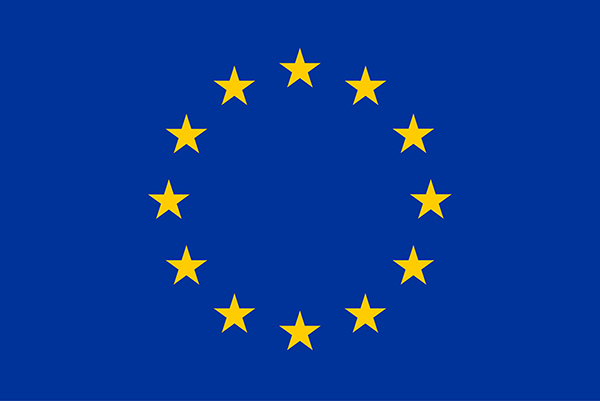
\includegraphics[width=10cm]{Images/euflag.jpg}
    \vspace*{0.5cm}\par
    {\fontsize{50}{60} \textbf{\thetitle}\par}
    \vspace*{0.2cm}
    {\fontsize{30}{30}\selectfont \textbf{Grundsätze  und Werte} \par}
    \vspace*{1cm}
    {\fontsize{24}{30}\selectfont{\theauthor} \\}
    {\fontsize{18}{30}\selectfont 593402 \par}
    {\fontsize{18}{22}\selectfont Wissenschaftliches Arbeiten mit Latex \par}
    \vspace*{1cm}
    
\includegraphics[width=3cm]{Images/htw_logo.jpg}
    \vspace*{1cm}
\end{titlepage}

% Inhaltsverzeichnis
\tableofcontents

% Kapitel
\chapter{Geschichte der EU}

Das Ende des 2. Weltkriegs bestimmt eine neue Zeit in Europa. Der Wunsch nach einem friedlichen Europa, wird nach zwei Weltkriegen in der ersten Hälfte des 20. Jahrhunderts, immer größer. Auf dem Schutt des verwüsteten Europas baut man in den darauf folgenden 13 Jahren, das Fundament aus dem die heutige Institution der Europäischen Union hervorgeht. Dieser komplexe Prozess wird oft bezeichnet als die europäische Integration\parencite[]{montanunion}.


\section{Gründung der NATO - April 1949}
Im April 1949 wird der Nordatlantikvertrag unterzeichnet von den USA, Kanada, Belgien, Dänemark, Frankreich, dem Vereinigtes Königreich, Island, Italien, Luxemburg, die Niederlande, Norwegen und Portugal. Damit wird eine zwischenstaatliche Sicherheitsallianz gebildet, die nach der europäischen Verwüstung nach dem zweiten Weltkrieg, erstmals wieder Stabilität und Sicherheit vermittelt. Dadurch wird Vertrauen und Zusammenarbeit gefördert und legt eine Grundlage für die zukünftige Zusammenarbeit vorallem zwischen den europäischen Gründungsmitgliedern.

\section{Europarat - Mai 1949}
\begin{wrapfigure}{r}{0.5\textwidth} 
    \centering
    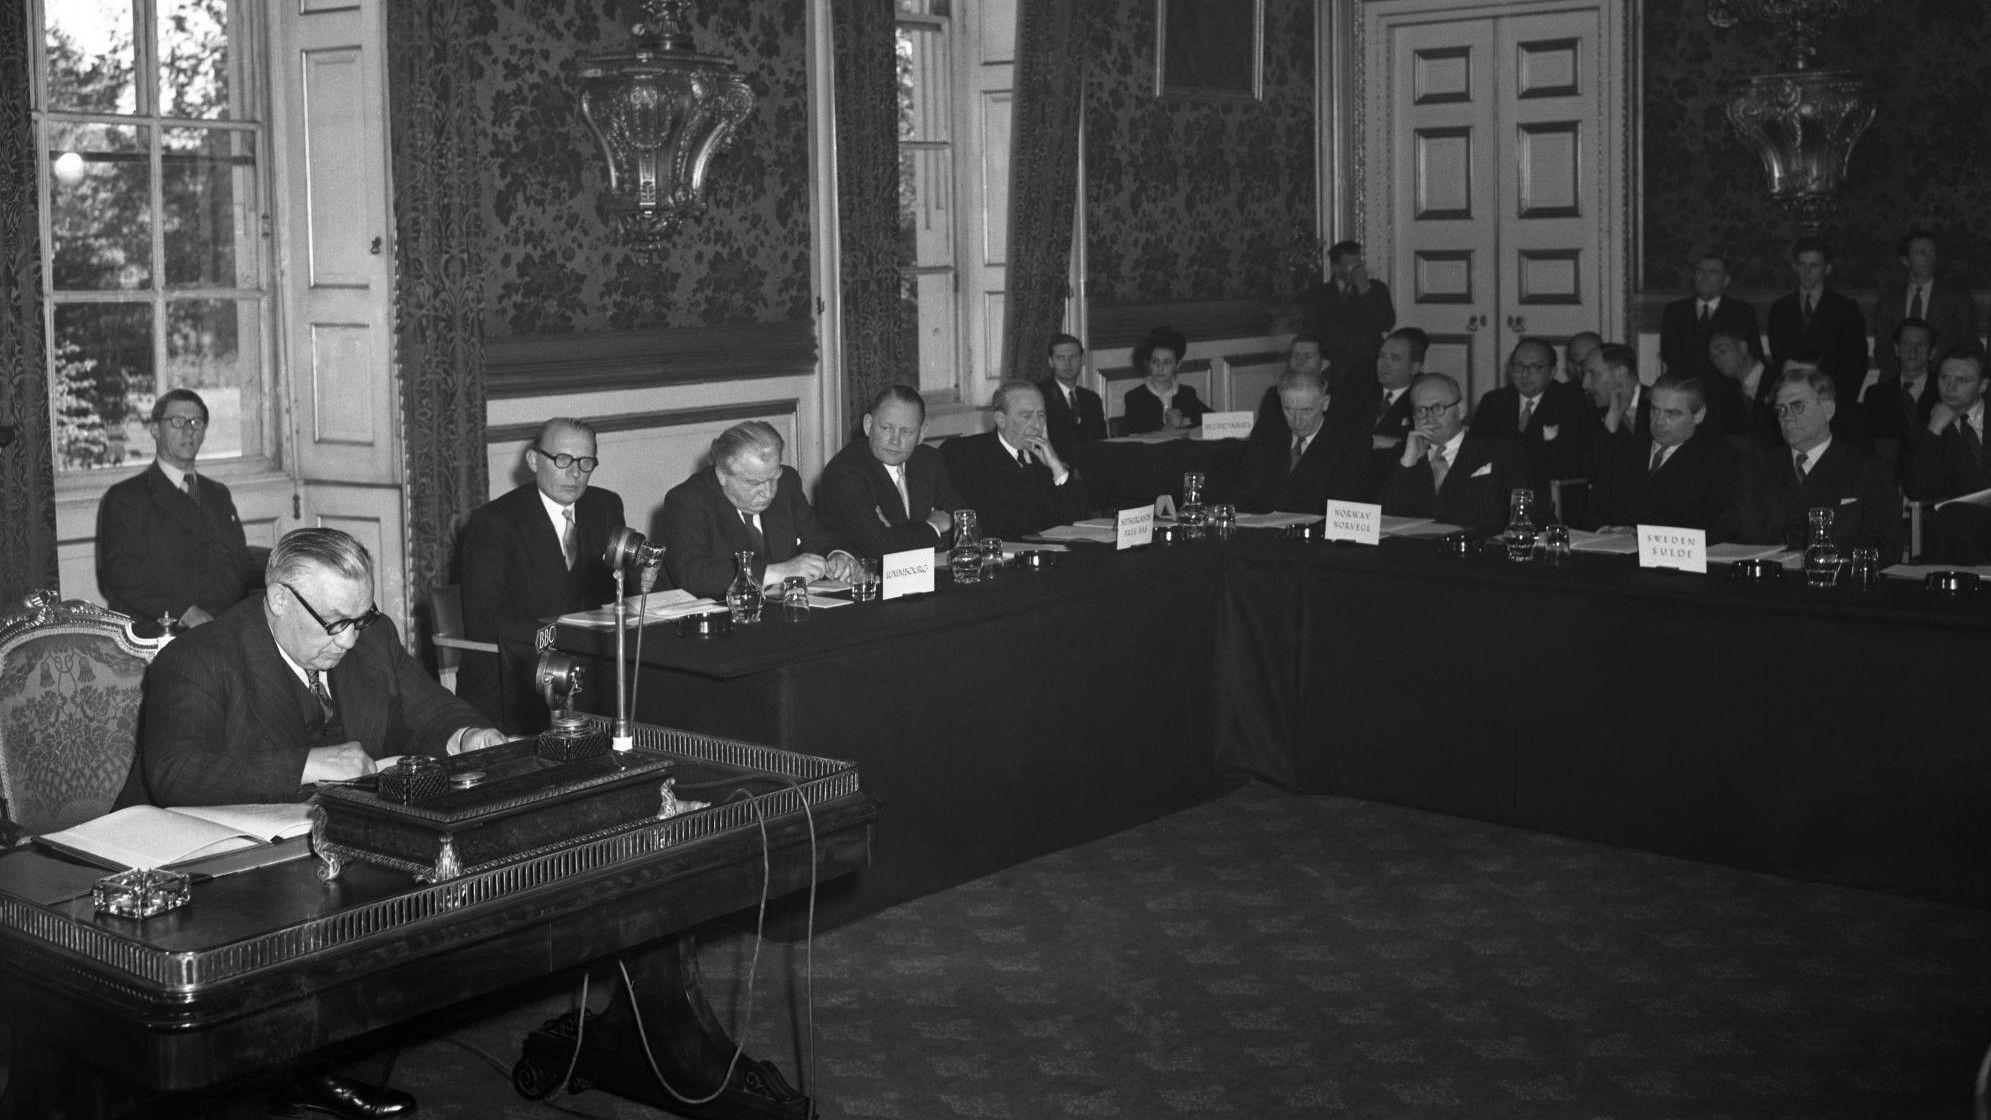
\includegraphics[width=0.41\textwidth]{Images/europarat.png} 
    \caption{Der britische Außenminister Ernest Bevin unterzeichnet das „Statut des Europarates“}
    \label{fig:wrap}
\end{wrapfigure}
Die älteste politische Institution europäischer Staaten ist der Europarat. Im Mai 1949 wird die Satzung im Londoner Zehnmächtepakt festgehalten und damit bekennen sich Belgien, Dänemark, Frankreich, Irland, Italien, Luxemburg, Niederlande, Norwegen, Schweden und das Vereinigten Königreich öffentlich zu Demokratie, Menschenrechten und Rechtsstaatlichkeit. Es wird 1950 die Europäische Menschenrechtskonvention beschlossen und 1953 tritt diese in Kraft \parencite[]{euConventionOfHumanRights-Plan}.



\section{Europäische Gemeinschaft für Kohle und Stahl - April 1951}
Der französische Außenminister Robert Schuman schlägt am 9. Mai 1950 den Plan vor die Kohle- und Stahlindustrie, beide essenziell in der Waffenherstellung, der Westeuropäischen Länder zu vereinen \parencite[]{Schuman-Plan}. Auf Grundlage des Schuman-Plans unterzeichnen Belgien, Deutschland, Frankreich, Italien, Luxemburg und die Niederlande im April 1951 einen Vertrag über die gemeinsame Kontrolle der Kohle und Stahl. 1952 tritt diese Vertrag in Kraft unter den Namen der Europäische Gemeinschaft für Kohle und Stahl(EGKS).

\section{Die Römischen Verträge - März 1957}
Nachdem scheitern der Gründung der Europäischen Verteidigungsgemeinschaft (EVG) und der Europäischen Politischen Gemeinschaft (EPG) im Jahre 1954, suchte man nach einer weiteren wirtschaftlichen Zusammenarbeit, die auf dem Erfolg der EKGS aufbaut. Auf der Konferenz von Messina 1955 beschloss man das Einsetzen eines Regierungsauschuss, unter Vorsitz von Paul-Henri Spaak, in dem die Grundlagen und Möglichkeiten eines gemeinsamen Marktes verhandelt werden sollen. Aufgrund des Berichts aus der Spaak-Kommission \parencite[]{Spaak-Bericht} einigten sich die 6 Staaten der EGKS  auf eine Vereinheitlichung des Gemeinsamen Marktes und der zivilen Nutzung der Atomenergie. Am 25. März 1957 wurden die Verträge zur Gründung der europäischen Wirtschaftsgemeinschaft (EWG) und der europäischen Atomgemeinschaft unterzeichnet. 

\subsection{Europäische Wirtschaftsgemeinschaft}
Der Vertrag zur Gründung der EWG wurde zuerst auf unbegrenzte Zeit geschlossen. Der Vertrag gehört inzwischen zu den primären Rechtsquellen innerhalb des Europarechts. Zur Gründung der EWG wurden sich auf folgende Ziele geeinigt\parencite[]{EWG}: 

\begin{itemize}
    \item Sicherung des sozialen und wirtschaftlichen Fortschritts
    \item Beseitigung europäischer Schranken, Abschaffung der Zölle
    \item Besserung der Lebens- und Beschäftigungsbestimmungen
    \item beständige Wirtschaftsausweitung, ausgewogener Handelsverkehr, redlicher
    Wettbewerb
    \item gemeinsame Handels-, Landwirtschafts- und Verkehrspolitik
    \item Wahrung von Frieden und Freiheit
    \item größere Stabilität, engere Beziehungen zwischen den Staaten
    \item freier Personen-, Dienstleistungs-, Kapital- und Warenverkehr
    \item Angleichung innerstaatlicher Rechtsvorschriften
    \item innere und äußere finanzielle Stabilität
\end{itemize}


\subsection{Europäische Atomgemeinschaft}
Auch dieser Gründungsvertrag wurde zunächst auf unbegrenzte Zeit geschlossen. Mit besonderen Bestrebungen von Louis Armand betonte der Spaak Bericht die Notwendigkeit die Forschungs- und Investitionsanstrengungen der Atomenergie zusammenzulegen. Insbesondere des wachsenden europäischen Energiebedarfs und der damaligen Hoffnung auf eine "friedliche Nutzung" der Kernenergie, war das Hauptziel von Euratom, die gemeinsame Entwicklung und Nutzung der Kernenergie in den Mitgliedstaaten zu koordinieren \parencite[]{Spaak-Bericht}.
\par
Die fünf großen Themengebiete der Atomgemeinschaft umfassen:

\begin{enumerate}
    \item Entwicklung der Forschung und Informationsaustausch
    \item Sicherheitsregeln und -kontrollen zum Schutz der Arbeiter und der Bevölkerung
    \item Entwicklung der Investitionen und gemeinsame Einrichtungen
    \item Versorgung mit Erzen und Kernbrennstoffen
    \item Einrichtung eines gemeinsamen Marktes auf dem Atomgebiet
\end{enumerate}

\section{Europäische parlamentarische Versammlung - März 1958}
Die Versammlung der EGKS wurde nach der Gründung der EWG und EAG zusammengelegt. Daraus entsteht in Straßburg die erste europäische parlamentarische Versammlung(Vorläufer des heutigen EU-Parlaments) bei der Robert Schuman zum Präsidenten gewählt wird. Diese Versammlung wird im März 1962 offiziell umbenannt in Europäisches Parlament.


\section{EG-Fusionsvertrag - April 1965}
Mit den Römischen Verträgen wurde auch beschlossen, dass sich die EGKS, EWG und EAG sich politische Organe teilten. Darunter waren ein gemeinsames Parlament, einen Gerichtshof und ein gemeinsamer Wirtschafts- und Sozialausschuss. Der Fusionsvertrag führte schließlich zur Zusammenlegung dieser Organe, indem die verschiedenen Ministerräte und Kommissionen zusammengeführt wurden. Damit war die Vereinheitlichung der Gemeinschaftsorgane abgeschlossen.

\section{Europäische Politische Zusammenarbeit - Dezember 1970}
Auf dem Gipfeltreffen der Staats- und Regierungschefs der Mitgliedsstaaten der europäischen Gemeinschaften wurde zuerst untersucht, die Außenpolitik der Mitgliedsstaaten anzugleichen. Ein darauffolgender Ausschuss, bestehend aus den Außenministern der Mitgliedsstaaten, diskutiert die stärkere außenpolitische Zusammenarbeit. Aus diesem Ausschuss entsteht ein Bericht der bekannt wird als Davignon-Bericht und als Grundlage der Europäischen Politische Zusammenarbeit (EPZ) gesehen wird. Im Dezember Die EPZ wird zunächst ohne eigene vertragliche Grundlage festgehalten und basiert auf freiwilliger Zusammenarbeit der beteiligten Regierungen. Die Befugnisse der EZP wurde durch Beschlüsse in Kopenhagen 1973 und in London 1981 weiter ausgebaut.

\section{Erweiterung auf 9 Mitgliedsstaaten - Januar 1973}
Zum 1. Januar 1973 treten Dänemark, Irland und das Vereinigte Königreich den europäische Gemeinschaften bei. Aufgrund dem andauerendem kalten Krieg erhoffte man sich durch die Erweiterung eine wirtschaftliche Verstärkung und mehr geopolitscher Bedeutung. Trotz anfänglicher Widerstände, vor allem seitens Frankreichs gegenüber dem britischen Beitritt, ebnete diese Erweiterung den Weg für eine tiefere und umfassendere europäische Zusammenarbeit.

\section{Europäischer Rat - Dezember 1974}
Nicht zu verwechseln mit dem Europarat, der bis heute nicht institutionel mit der EU verbunden ist, ist der europäische Rat. 
\par 
Entsprungen aus informellen Treffen der Staats- und Regierungschefs der EWG in den 1960er Jahren, dienten diese Treffen zunächst den Austausch von Meinungen und der Koordinierung politischer Initiativen. Der Gipfel von Paris im Dezember 1974 markierte die Geburtsstunde des Europäischen Rates, der als informelles Forum für regelmäßige Treffen der Staats- und Regierungschefs der EWG-Mitgliedstaaten etabliert wurde. Unter den französischen und deutschen Regierungschefs  Valéry Giscard d’Estaing und Helmut Schmidt spielte der europäische Rat eine entscheidende Rolle bei der Weiterentwicklung der europäischen Integration, insbesondere bei der Verabschiedung wichtiger Verträge wie der einheitlichen Europäischen Akte (1986).

\section{1. Wahl des Parlaments - Juni 1979}
Zuvor wurden die Mitglieder des Parlaments von ihren nationalen Parlamenten abgeordnet, doch im Juni 1979 durften die Bürger der Mitgliedsstaaten zum ersten Mal die Mitglieder des Europäischen Parlaments selbst wählen. 

\section{Erweiterung auf 10 Mitgliedsstaaten - Januar 1981}
Nach dem Ende des Militärregimes im Jahr 1974 und der Wiederherstellung der Demokratie konnte Griechenland 1981 den Europäischen Gemeinschaften beitreten.

\section{Erweiterung auf 12 Mitgliedsstaaten - Januar 1986}
Portugal und Spanien treten den europäischen Gemeinschaften bei.

\section{Einheitliche europäische Akte - Februar 1986}
Nach langen Debatten, die Instutionen und Organe der drei großen europäischen Gemeinschaften zu Reformieren, kam es im europäischem Rat 1985 zu einer Abstimmung, die zum einem der EPZ eine vertragliche Grundlage geben sollte und die Schaffung eines Fahrplans für einen gemeinsamen Binnemarkt beschließen sollte. Daraus folgend wurde ein Änderungsvertrag der Gemeinschaften verfasst der im Februar von allen 12 Mitgliedsstaaten unterschrieben wurde. Essenzielle Neuerungen waren:

\begin{itemize}
    \item Abbau von Handelshemnissen und die Vollendung eines Binnenmarkts bis 1992
    \item Reformierung von Entscheidungsprozessen durch die Einführung des qualifizierten Mehrheitsbeschlusses
    \item Stärkung des europäischen Parlaments durch mehr Einfluss auf die Gesetzgebung
    \item Vertrag für eine gemeinsame europäische Außenpolitik
\end{itemize}

\chapter{Gründung der EU}

\section{Vertrag von Maastrich - Februar 1992}
Der am 7. Februar 1992 unterzeichnete und am 1. November 1993 in Kraft getretene Vertrag von Maastricht, offiziell bekannt als Vertrag über die Europäische Union, markiert einen entscheidenden Wendepunkt in der Geschichte der europäischen Integration. Er gilt als die Geburtsstunde der Europäischen Union (EU) in ihrer modernen Form. Das Vertragswerk ersetzte die vorherigen Römischen Verträge und führte die Europäische Union als übergeordnete politische und wirtschaftliche Instanz ein der bestehenden Europäischen Gemeinschaften (EG), der Europäischen Wirtschaftsgemeinschaft (EWG) und Euratom. Ein zentraler Aspekt des Vertrags war die Einführung der sogenannten \hyperref[tab:eu_saeulen]{drei Säulen der Europäischen Union}, eine Struktur, die die verschiedenen Politikbereiche und Zuständigkeiten der EU definierte. Dazu legte der Vertrag auch den Grundstein für die Einführung des Euros in den Folgejahren.
Die Struktur der drei Säulen, wie in der \hyperref[tab:eu_saeulen]{dargestellten Tabelle}, illustriert die Komplexität und den Umfang der des Vertragswerks. Er legte den Grundstein für die Weiterentwicklung der EU zu einer politischen Union.

\begin{table}[H]
\centering
\begin{tabular}{|p{5cm}|p{5cm}|p{5cm}|}
    \hline
    \rowcolor{hellblau}
    \multicolumn{1}{|c|}{\textbf{1. Säule}} & \multicolumn{1}{|c|}{\textbf{2. Säule}} & \multicolumn{1}{|c|}{\textbf{3. Säule}} \\ \hline
    \textbf{Europäische \newline Gemeinschaften (EG)} & \textbf{Gemeinsame Außen- und \newline Sicherheitspolitik (GASP)} & \textbf{Zusammenarbeit der Polizei und Justiz (PJZS)} \\ \hline
        
\textbf{EG:}
{\renewcommand{\labelitemi}{$\bullet$}
\begin{itemize}[leftmargin=*]
    \item Agrarpolitik
    \item Zollunion 
    \item Binnenmarkt
    \item Strukturpolitik
    \item Handelspolitik
    \item Wirtschaftsunion
    \item Währungssunion
    \item Bildung und Kultur
    \item Forschung und Umwelt
    \item Gesundheitswesen
    \item Verbraucherschutz
    \item Sozialpolitik
\end{itemize}}

\vspace{0.2cm}

\textbf{Euratom:} 
{\renewcommand{\labelitemi}{$\bullet$}
\begin{itemize}[leftmargin=*]
    \item Zusammenarbeit im Bereich Kernenergie
\end{itemize}}

&

\textbf{Außenpolitik:}
{\renewcommand{\labelitemi}{$\bullet$}
\begin{itemize}[leftmargin=*]
    \item Gemeinsame Positionen
    \item Friedenserhaltung
    \item Menschenrechte
    \item Demokratie
    \item Hilfe für Nicht-EU-Staaten
\end{itemize}}

\vspace{0.2cm}

\textbf{Sicherheitspolitik:}
{\renewcommand{\labelitemi}{$\bullet$}
\begin{itemize}[leftmargin=*]
    \item Gemeinsame Vorgehen
    \item Kampf gegen Terrorismus
    \item Gemeinsame Truppen
\end{itemize}}

&

\textbf{Polizei und Justiz:}
{\renewcommand{\labelitemi}{$\bullet$}
\begin{itemize}[leftmargin=*]
    \item Kampf gegen die organisierte Kriminalität (z.B. Drogen, Menschenhandel)
    \item Einwanderungspolitik
    \item Asylpolitik
    \item Zusammenarbeit in Zivil- und Strafprozessen
    \item Polizeiliche Zusammenarbeit
    \item Hilfe für Nicht-EU-Staaten
\end{itemize}}
\\
\hline

\end{tabular}
\caption{Die drei Säulen der Europäischen Union}
\label{tab:eu_saeulen}
\end{table}

\section{Der Euro als gemeinsame Währung - Mai 1998}
Mit der Gründung der europäischen Zentralbank im Juni 1998 war einer der letzten entscheidenden Schritte getan um die Einführung des Euros zu gewährleisten. Das Vorgehen und die Einführung des Euros wurde stark kritisiert und wäre fast wie auch schon vorherige Vorhaben der europäischen Integration von der Öffentlichen Meinung diktiert ins Wasser gefallen\parencite[]{Interstests-and-Integration}. Im Mai 1998 entschlossen sich entgegen der Öffentlichen Meinung die Staats- und Regierungschefs der Europäischen Gemeinschaften die Einführung des Euros zu beschließen. Im nachhinein bekannt geworden mit welcher Härte sich gegen die Öffentlichkeit gewandt wurde, ist das Zitat von Helmut Kohl: "In einem Fall war ich wie ein Diktator, siehe Euro."  \parencite[]{Helmut-Kohl-Zitat}.

Banken und Finanzmärkte rechneten schon ab 1999 mit dem Euro. Die Ausgabe als Bargeld an die Bürger begann am 1. Januar 2002 in 12 Ländern und damit erfolgte die größte Bargeldumstellung der Geschichte. Von den aktuell 27 Mitgliedsländern (Stand 10. März 2025) verwenden 20 Länder den Euro und befinden sich in der sogenannten Eurozone.

\begin{figure}[htbp]
    \centering
    \subfloat[Zeitverlauf EG und EU]{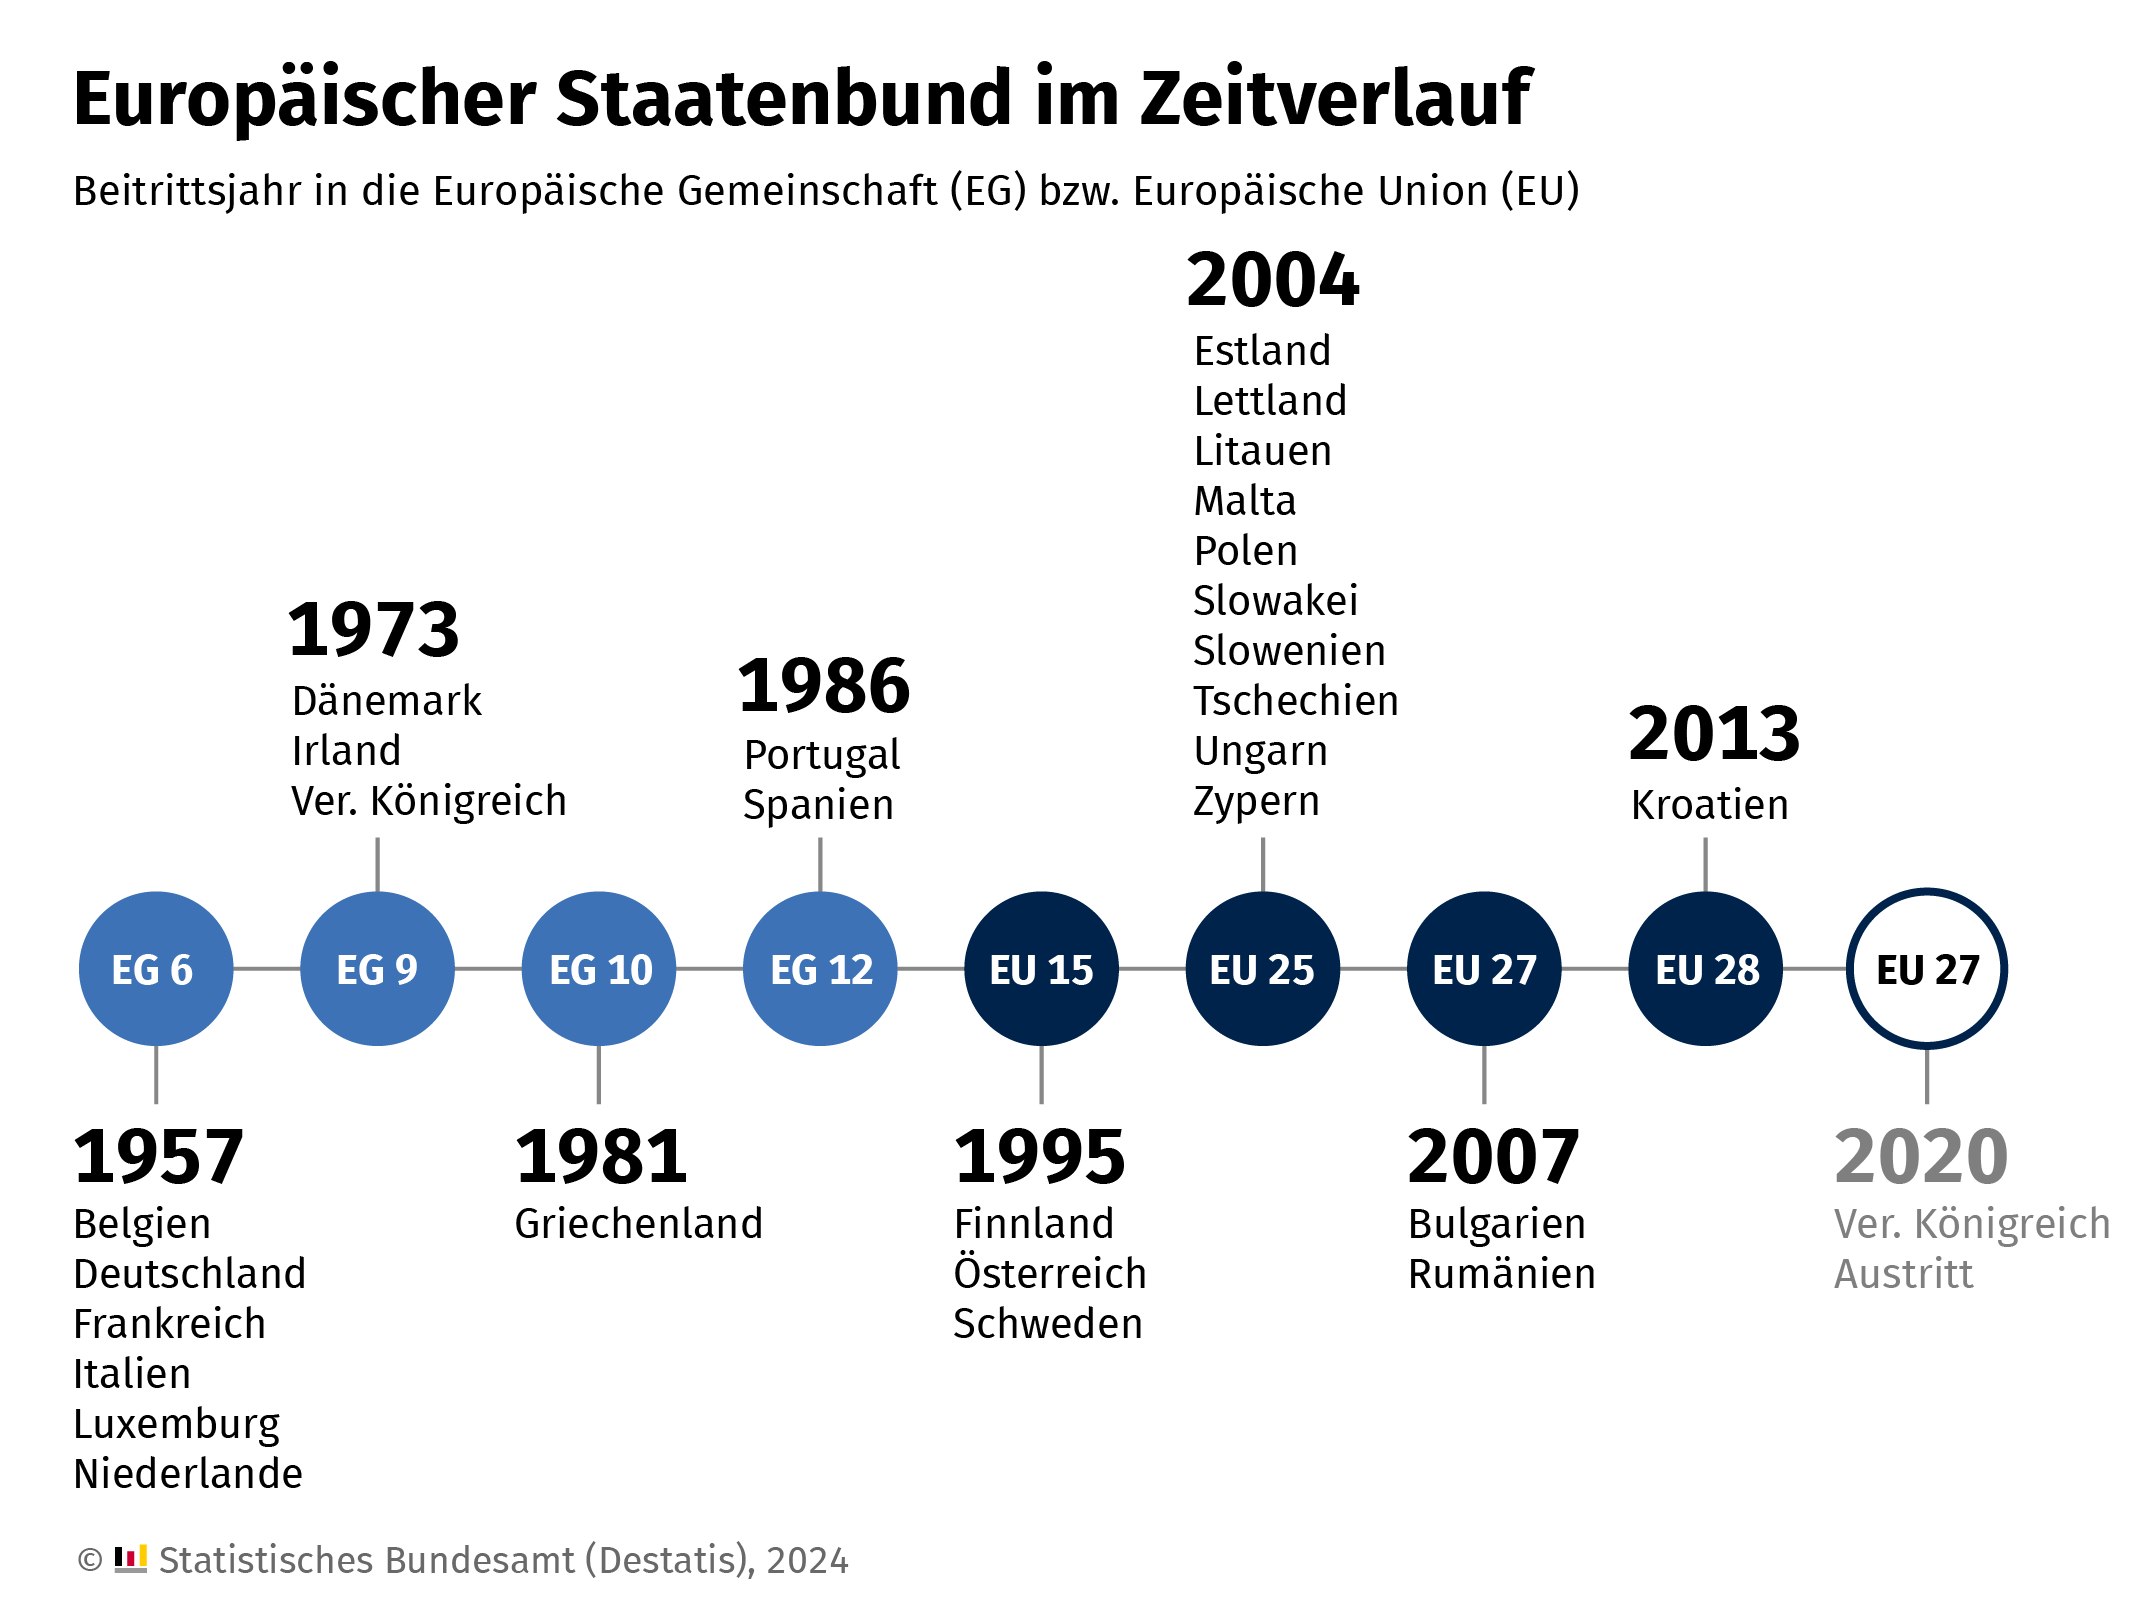
\includegraphics[width=0.5\textwidth]{Images/zeitverlauf_eu.png}} % Ersetze durch dein Bild
    \subfloat[Zeitverlauf Eurozone]{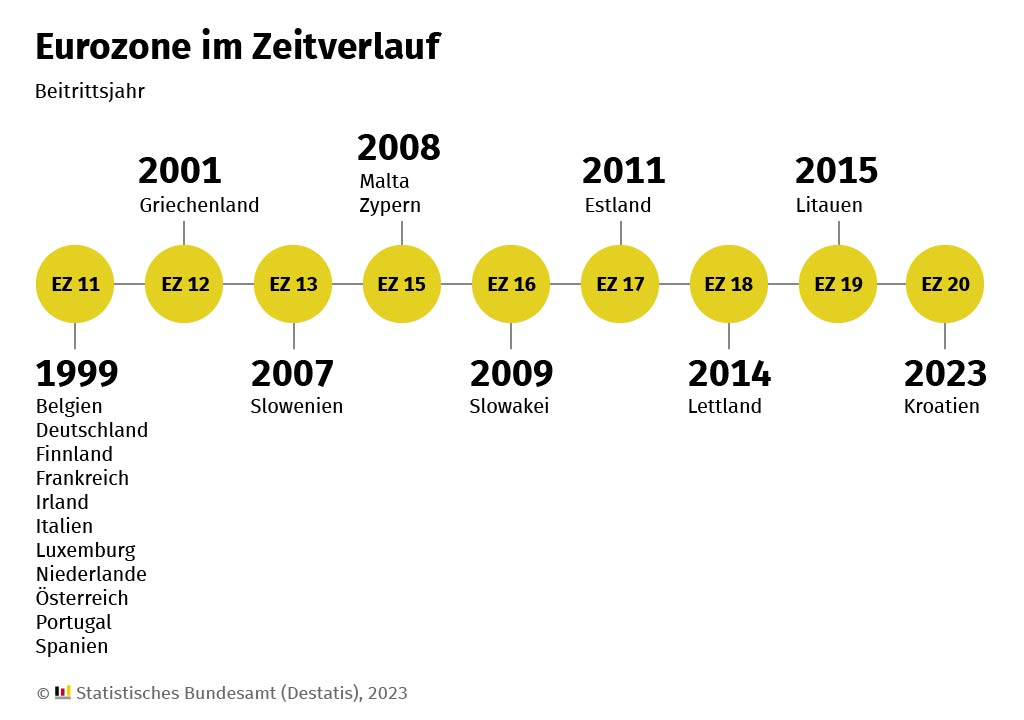
\includegraphics[width=0.53\textwidth]{Images/zeitverlauf_eurozone.png}} % Ersetze durch dein Bild
    \caption{Verlauf der europäischen Staatenbündnisse und der Eurozone}
    \label{fig:subfigure}
\end{figure}

\section{Vertrag von Amsterdam - Juni 1997}
Der Vertrag von Amsterdam, unterzeichnet 1997, trat 1999 in Kraft, modernisierte die EU mit Blick auf die bevorstehende Osterweiterung. Er stärkte das Europäische Parlament, verbesserte die Zusammenarbeit in Justiz und Inneres durch die Integration des Schengen-Besitzstands, wertete die Gemeinsame Außen- und Sicherheitspolitik auf und sorgte für mehr Bürgernähe durch verbesserten Grundrechtsschutz und Vertragsvereinfachungen. Wichtige Fortschritte im Bereich der Grundrechte wie die Gleichstellung von Männern und Frauen wurden ausdrücklich als Ziel der EU festgeschrieben, und es wurden Bestimmungen zur Bekämpfung von Diskriminierung aufgenommen.

\vspace{1cm}

\section{Vertrag von Nizza - 2003}
Die Hauptaufgabe dieses Vertrags war die Umsetzung der Erweiterung der EU um 10 Mitgliedsländer vorzubereiten. 
Die wichtigsten Aspekte des Vertrags umfassen:


\begin{description}
    \item[]
\end{description}


\begin{itemize}
    \item Neugewichtung der Stimmen im EU-Rat vorbereitend auf die bevorstehende geänderte Bevölkerungsstruktur. Dadurch sollen zukünftige Entscheidungsprozesse effizent gestaltet werden
    \item Anpassung der Größe der europäichen Kommission in ihrer Größe und Zusammensetzung
    \item Ausdehnung von Abstimmungen mit qualifizierte Mehrheit
    \item Reformen an der Struktur des europäischen Gerichtshofs
    \item Anpassungen um eine verstärkte Zusammenarbeit besser zu Ermöglichen
\end{itemize}

\section{Vertrag von Lissabon - 2007}
Obwohl unterzeichnet 2007, trat der Vertrag erst 2009 in Kraft und reformierte damit das bestehende Vertragswerk der Europäischen Union. Die Ziele waren es die EU demokratischer, handlungsfähiger und transparenter zu machen. 

Das komplexe drei Säulen Modell der EU wurde abgeschafft. Dadurch wurde die EU transparenter und die Entscheidungsfindung wurde vereinfacht und beschleunigt.
Es wurde zudem das Amt des Hohen Vertreters für die gemeinsame Außen- und Sicherheitspolitik und das Amt des Ratspräsidenten geschaffen. Die EU erhielt eine einheitliche Rechtspersönlichkeit, was ihre Handlungsfähigkeit auf internationaler Ebene verbesserte. Die Charta der Grundrechte der Europäischen Union wurde rechtsverbindlich, wodurch der Schutz der Grundrechte in der EU gestärkt wurde. Zum ersten Mal wurde auch ein Regelwerk für den Austritt eines Mitgliedstaates aus der EU in den Vertrag aufgenommen.


\chapter{Grundsätze, Werte}
\section{EU Vertrag}
Die Vorgänger der EU kamen zuerst zusammen für ein wirtschaftliches Interesse. Daraus entwickelte sich unteranderem die Wirtschaftgemeinschaft. Heutzutage ist die EU mehr als nur eine Wirtschaftsgemeinschaft und vorallem auch eine Wertegemeinschaft. Durch den EU-Vertrag und dessen Charta sind gemeinsame Werte und wirtschaftliche vertraglich festgehalten und bindend.
Der Artikel 2 des EU-Vertrags fasst deutlich zusammen welche Werte die EU vertritt und wofür sich jedes Mitgliedsland verpflichtet\parencite[]{eu-vertag}. Diese werden in diesem Kapitel im Detail behandelt.

\textit{Die Werte, auf die sich die Union gründet, sind die Achtung der Menschenwürde, Freiheit, Demokratie,
Gleichheit, Rechtsstaatlichkeit und die Wahrung der Menschenrechte einschließlich der Rechte
der Personen, die Minderheiten angehören. Diese Werte sind allen Mitgliedstaaten in einer Gesellschaft
gemeinsam, die sich durch Pluralismus, Nichtdiskriminierung, Toleranz, Gerechtigkeit, Solidarität
und die Gleichheit von Frauen und Männern auszeichnet.}

\section{Frieden}
\begin{wrapfigure}{r}{0.5\textwidth} 
    \centering
    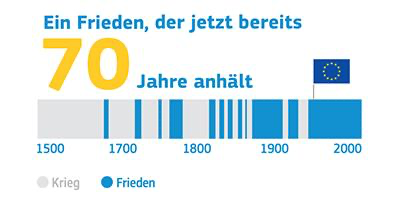
\includegraphics[width=0.45\textwidth]{Images/frieden.png} 
    \caption{Zeitstrahl für Frieden in Europa}
    \label{fig:wrap}
\end{wrapfigure}
Nach dem Ende des zweiten Weltkriegs entstand sich ein Leitgedanke, der sich in den darauffolgenden ersten Staatenbündnissen wiederspiegelt: Die Herrschaft der Stärke des Rechts vor dem Recht des Stärkeren. Gewalt ist kein Mittel der Politik. Dieser Leitgedanke ist seit über 70 Jahre Teil der europäischen Integration und etablierte, damit erfolgreich einen kriegsfreien Kontinent bis zum russischen Angriffskrieg auf die Ukraine 2022. 

\textbf{Art. 3 Abs. 1 EU-Vertrag:}
\newline
\textit{Ziel der Union ist es, den Frieden, ihre Werte und das Wohlergehen ihrer Völker zu fördern.}

Die EU setzt sich weltweit für Demokratie und Menschenrechte ein und ist in eine wichtige internationale diplomatischen Rolle gewachsen. Für diese Bemühungen wurde die EU 2012 für den Friedensnobelpreis ausgezeichnet. Das norwegische Nobelkomitee begründete seine Entscheidung mit der stabilisierenden Rolle der EU bei der Umwandlung Europas „von einem Kontinent der Kriege zu einem Kontinent des Friedens“. 



\section{Achtung der Menschenwürde}
Ein zentraler Aspekt ist die Achtung der Menschenwürde. Dies bedeutet, dass jeder Mensch unabhängig von seiner Herkunft, seinem Geschlecht, seiner Religion oder seiner Weltanschauung ein unveräußerliches Recht auf Leben, Freiheit und Sicherheit hat. Die EU verpflichtet sich, die Menschenwürde zu schützen und zu fördern, und lehnt jegliche Form von Diskriminierung und Misshandlung ab.

\section{Freiheit}
Ein weiterer großer Aspekt ist die Bewegungsfreiheit. Diese ermöglicht es jedem EU Bürger überall in der Union zu arbeiten, leben und sich frei zu bewegen. Angebote wie das Erasmus+ Programm ermöglichen seit mehreren Jahrzehnten Austauschprogramme für über 10 Millionen Teilnehmern.

Jedes Mitgliedsland hat sich dazu verpflichtet persönliche Freiheiten zu wahren und zu schützen. Diese sind in der Charta der Grundrechte der Europäischen Union verankert:

\begin{description}
    \item[Recht auf Freiheit und Sicherheit]
    \item[Achtung des Privat- und Familienlebens]
    \item[Schutz personenbezogener Daten]
    \item[Recht, eine Ehe einzugehen und eine Familie zu gründen]
    \item[Gedanken-, Gewissens- und Religionsfreiheit]
    \item[Freiheit der Meinungsäußerung und Informationsfreiheit]
    \item[Versammlungsfreiheit]
    \item[Freiheit der Kunst und der Wissenschaft]
    \item[Recht auf Bildung]
    \item[Berufsfreiheit und Recht zu arbeiten]
    \item[Unternehmerische Freiheit]
    \item[Eigentumsrecht]
    \item[Asylrecht]
    \item[Schutz bei Abschiebung, Ausweisung und Auslieferung]
\end{description}

\section{Demokratie}
Die EU selbst ist eine demokratische Institution und alle Mitgliedsländer verpflichten sich zur Demokratie und demokratischen Werten. Das gewählte EU Parlament und die national gewählten Parlamente bilden einen großen Teil des Gesetzgebungsprozesse. Die Rechtsstaatlichkeit ist ein weiteres wesentliches Prinzip der EU. Sie garantiert, dass alle Entscheidungen auf dem Gesetz beruhen und dass die Bürgerinnen und Bürger Zugang zu unabhängigen Gerichten haben. Die Rechtsstaatlichkeit schützt vor Willkür und gewährleistet, dass die Gesetze fair und transparent angewendet werden.

\section{Gleichheit}
Als weiterer Kernaspekt ist die Gleichheit. Das bedeutet dass alle Bürgerinnen und Bürger vor dem Gesetz gleich sind und die gleichen Rechte und Pflichten besitzen. Diskriminierung aufgrund von Geschlecht, Rasse, ethnischer Herkunft, Religion, Weltanschauung, Behinderung, Alter oder sexueller Orientierung ist verboten.

\chapter{Erfolge und Errungschaften}
\section{Klimaschutz}
Die EU hat sich als Vorreiter im Kampf gegen den Klimawandel positioniert und internationale Abkommen wie das Pariser Klimaabkommen maßgeblich mitgestaltet. Neben diesem Abkommen wurde der Europäische Green Deal beschlossen. Diese umfassende Strategie zielt darauf ab, Europa bis 2050 zum ersten klimaneutralen Kontinent der Welt zu machen. Der Green Deal umfasst eine breite Palette von Maßnahmen, darunter die Reduzierung von Treibhausgasemissionen durch den Ausbau erneuerbarer Energien, die Steigerung der Energieeffizienz, die Förderung nachhaltiger Mobilität und die Umsetzung einer Kreislaufwirtschaft.

\begin{figure}[H]
    \centering
    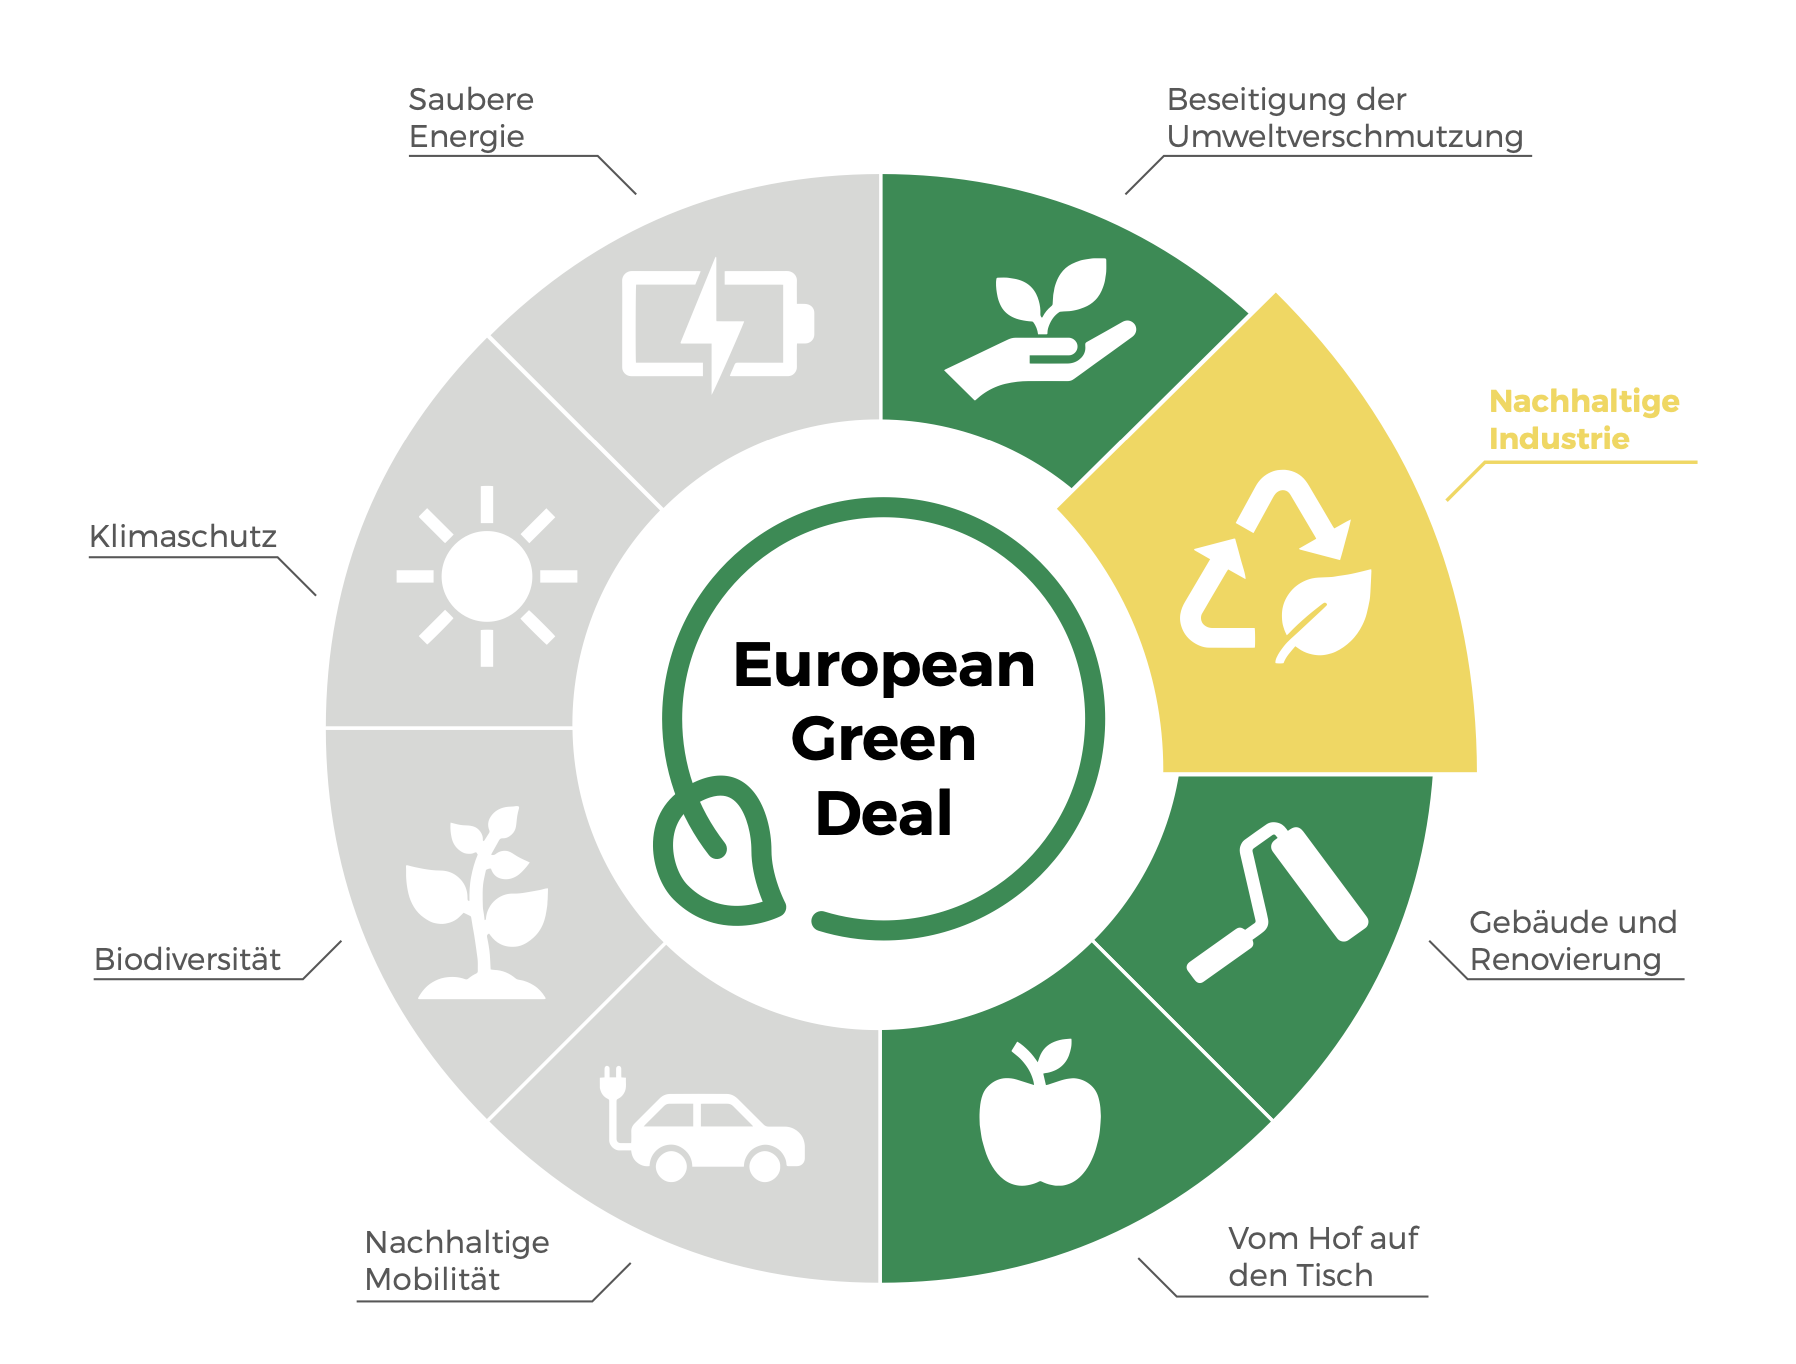
\includegraphics[width=0.8\textwidth]{Images/green_deal.png} 
    \caption{Aspekte des Green Deals}
    \label{fig:green_deal}
\end{figure}



\section{Humanitäre Hilfe und Entwicklungshilfe}
Die EU und ihre Mitgliedstaaten sind weltweit die größten Geldgeber für die Entwicklungshilfe und leisten seit 1992 einen wichtigen Beitrag zur Armutsbekämpfung, zur Förderung von Bildung und Gesundheit sowie zur Unterstützung von Krisengebieten. Die Projekte der EU und deren Kooperationen mit verschiedensten NGOs und der UN haben bisher Millionen von Menschen in über 110 Ländern erreicht und ein Netzwerk errichtet, welches noch in über 40 Ländern aktiv ist.

\begin{figure}[H]
    \centering
    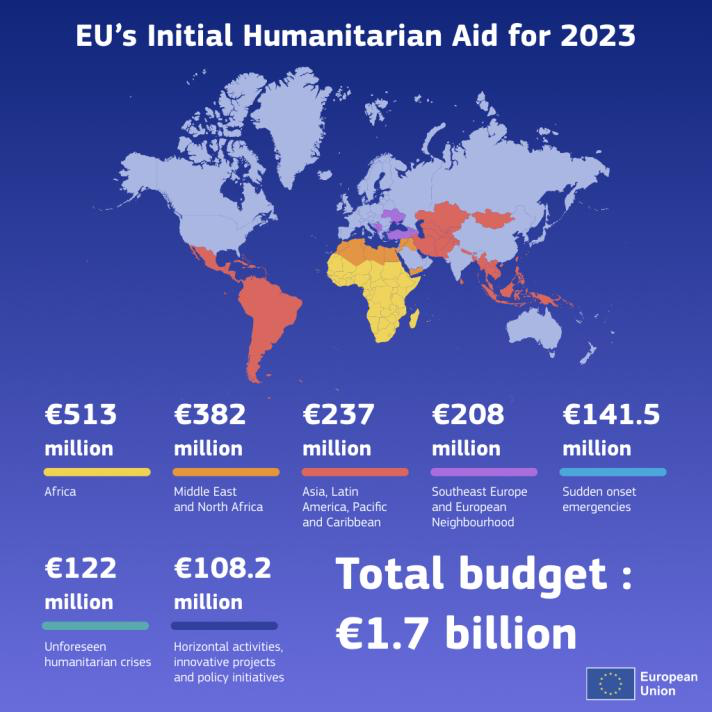
\includegraphics[width=0.6\textwidth]{Images/hu_aid.png} 
    \caption{Budget der EU für Humanitäre Hilfe}
    \label{fig:hu_aid}
\end{figure}

\section{Förderung der Demokratie und von Menscherechten}
Die EU hat sich in den letzten Jahrzehnten verstärkt als globaler Akteur für die Förderung von Demokratie, Rechtsstaatlichkeit und Menschenrechten etabliert. Als einer der weltweit größten Wirtschafträume können durch Sanktionen und Handelsverbote auch auf wirtschaftlicher Ebene Druck auf Länder aufbauen, die Menschenrechte verletzten(siehe zuletzt Russland Ukraine Krieg). Die EU tritt auch in eine diplomatische Rolle und vermittelt zwischen Konfliktparteien. Ein konkretes Beispiel in Europa war zum Beispiel die EU maßgeblich an der Bewältigung des Serbien-Kosovo Konflikt beteiligt durch Friedenmissionen, Bereitstellung Humanitärer Hilfe und als Vermittler im Dialog zwischen den Konfliktparteien zu Agieren. 

% Abbildungsverzeichnis
\listoffigures
% Tabellenverzeichnis
\listoftables

\printbibliography

\end{document}